\newpage
\chapter{Experiments}
\label{sec:experiments}
\hl{SECTION UNDER CONSTRUCTION}\\
This chapter describes the setup of the experiments executed. First the data sets used in the experiments are described. Then the measures and the setup of the experiments are introduced.\\
The experiments shall provide information, which is not given in Saenko \& Kotenko \cite{saenko2012design}. In particular how parameters can be set and how the objectives of the role models evolve and impact other objectives. Also the EA is executed on datasets commonly used in role mining research.

\section{Data Sets}
\subsection{Real Datasets}
In many research papers the same datasets are used for performance evaluation of role mining algorithms. Table \ref{tab:realDatasets} lists some of these data sets and their components. The authors of \cite{Ene} obtained these datasets from Cisco firewalls and the Lotus Domino server of the Hewlett Packard (HP) networks. The healthcare dataset was collected from the US Veteran’s Administration.
\begin{table}
    \centering
    \begin{tabular}{|l|l|l|l|}
        \hline
        \rowcolor{myGray} 
        \textbf{Dataset} & \textbf{Users} & \textbf{Permissions} & \textbf{User Permission Assignments} \\ \hline
        healthcare       & 46             & 46                   & 1486                                 \\ \hline
        domino           & 79             & 231                  & 730                                  \\ \hline
        emea             & 35             & 3046                 & 7220                                 \\ \hline
        apj              & 2044           & 1146                 & 6841                                 \\ \hline
        firewall-1       & 365            & 709                  & 31951                                \\ \hline
        firewall-2       & 325            & 590                  & 36428                                \\ \hline
        americas-small   & 3477           & 1587                 & 105205                               \\ \hline
    \end{tabular}
    \caption{Real Datasets}
    \label{tab:realDatasets}
\end{table}
In Xu \& Stolter\cite{Xu} the authors created an algorithm to generate user attribute information on the datasets in table \ref{tab:realDatasets}.\hl{More details}

\subsection{Synthetic Datasets}
Some papers are providing data generators for synthetic datasets for the performance evaluation of the various role mining algorithms. The data generator in Vaidya et al.\cite{Vaidya:2006:RMR:1180405.1180424} takes as input the number of users, permissions and roles to generate a pair of User-Role-Assignment and Role-Permission-Assignment matrices. Combining these two matrices, the corresponding User-Permission-Assignment matrix is obtained.\\
\iffalse In the data generator introduced in [Lu et al. 2014]...\\
"In [Lu et al. 2014], several sets of synthetic data of varying parameters are used. The data generator takes as input the number of users and permissions, density of 1s in the PA, density of 1s in the UA and the noise level to produce the UA and PA matrices."\fi
These data generators only consider users, permissions and their assignment to each other. They do not consider user attribute information. Due to this a new synthetic data generator was created for this thesis, where the dimensions of users and permissions can be defined. The data generator is based on a reversed role-engineering process and generates users, roles, rules, user-role matrix, role-permission matrix, user-permission matrix and a user-permission matrix with noise.

\begin{itemize}
    \item \textbf{Generation of users}\\
    Given a user count $u$ and a list of user attributes $attr$ containing a list of user attribute values each, $u$ users are generated. A user is described by a list of user attributes, which have a specific user attribute value assigned. For example:\\
    \storestyleof{itemize}
    \begin{listliketab}
        \begin{tabular}{ll}
            Given   &  $attr$ = [$OrganizationalUnit$,$Location$,$EmployeeType$]\\
            where   &  $OrganizationalUnit$ = [$HumanResources$,$Sales$,$Motor$],\\
                    &  $Location$ = [$Denmark$, $Germany$, $US$] and\\
                    &  $EmployeeType$ = [$Internal$,$External$]\\
        \end{tabular}
    \end{listliketab}\\
    An user can be generated as follows: $user_1$ = [$Sales$,$Denmark$,$Internal$]. An additional parameter for a usertype count $t$ determines how many different users can exist. This ensures that users with the same user attributes can occur several times.
    
    \item \textbf{Generation of roles}\\
    Given a permission count $p$ and a role count $r$, $r$ roles are generated, which are described by a set of permissions from the range [1;$p$]. For example given $p$=7 a role can be: $role_1$ = \{$1$,$5$,$7$\}. A parameter $max_p$ limits how often a permission can occur in all $r$ roles. Additionally a configuration list $conf_p$ can regulate the density of roles. A configuration list entry contains 1) a percentage of all roles, which are affected by this configuration entry 2) the minimum count of permissions the role must have and 3) the maximum count of permissions the role must have. For example the configuration list [(0.2,10,20),(0.8,1,5)] would describe the configuration that 20\% of the $r$ roles must have between 10 and 20 permissions and the other 80\% of the $r$ roles must have between 1 and 5 permissions.
    
    \item \textbf{Generation of rules}\\
    \hl{UPDATE}
    Given a role count $r$ and a list of user attributes $attr$ containing a list of user attribute values each, $r$ rules are generated (a rule for each role). A rule is a list of user attributes, which have no, one or several user attribute values assigned. For example given the user attributes $attr$ from above, $rule_1$ = [\{$HumanResources$\}, \{$Denmark$,$Germany$\}, \{\}] would describe the rule $HumanResources \wedge (Denmark \vee Germany)$. A parameter for the maximal condition count $cond_{max}$ configures how many user attributes can be filled with values. The example $rule_1$ has currently two conditions: One for $OrganizationalUnit$ and one for $Location$.\\
    This rule is assigned to a role. Rules are generated until:
        \subitem \textbullet \space each role has a rule assigned
        \subitem \textbullet \space each generated user is meeting one rule
        \subitem \textbullet \space each rule is met by at least one user
\end{itemize}
Since users and roles have been generated before, the rules can be applied to create the following outputs:
\begin{itemize}
    \item \textbf{User-role matrix}\\
    The User-role matrix is a boolean matrix, where the rows are users and the columns are roles. A "1" in the matrix would mean that the user (row) is assigned to a the role (column). The users get those roles assigned, which have a rule assigned the user is fullfilling. For example $user_1$ would not fulfill $rule_1$, since the first condition for OrganizationalUnit is not met. The user $user_2$ = [$HumanResources$,$Denmark$,$Internal$] on the other hand would met the conditions in $rule_1$ and would therefore get get according role assigned.
    \item \textbf{Role-permission matrix}\\
    The Role-permission matrix is a boolean matrix, where the rows are roles and the columns are permissions. A "1" in the matrix would stand for that the role (row) is containing the permission (column). The matrix is generated from the generated roles.
    \item \textbf{User-permission matrix}\\
    The User-permission matrix is a boolean matrix, where the rows are users and the columns are permissions. A "1" in the matrix would imply that the user (row) is has the permission (column). The matrix is generated from the matrix multiplication of the User-role matrix and the Role-permission matrix.
    \item \textbf{User-permission matrix with noise}\\
    Given two parameters for noise, random bits in the User-permission matrix are flipped. The first parameter is the probability that a user-permission-relation is removed ("1" flipped to "0") and the second parameter is the probability that a user-permission-relation is added ("0" flipped to "1").
\end{itemize}
Three datasets have been generated with the data generator in order to execute experiments with fitness functions $F_{basic\_INT}^{min}$ \eqref{eq:FBasicMin_INT} and $F_{edge\_INT}^{min}$ \eqref{eq:FEdgeMin_INT}. The synthetic datasets are listed in table \ref{tab:syntheticDatasets}.
\begin{table}
    \centering
    \begin{tabular}{|l|c|c|c|c|}
        \hline
        \rowcolor{myGray} 
        \textbf{Dataset} & \textbf{Users} & \textbf{Permissions} & \textbf{User Permission Assignments} & \textbf{Roles}\\ \hline
        1       & 10    & 10   & 100    & 4\\ \hline
        2       & 50    & 50   & 2500   & 15\\ \hline
        3       & 100   & 100  & 10000  & 25\\ \hline
    \end{tabular}
    \caption{Synthetic Datasets}
    \label{tab:syntheticDatasets}
\end{table}
A visualization of synthetic dataset 1 and the healthcare dataset can be seen in Figure \ref{fig:dataset1} and \ref{fig:healthcare}.

\afterpage{
    \begin{figure}[!htb]
        \centering
        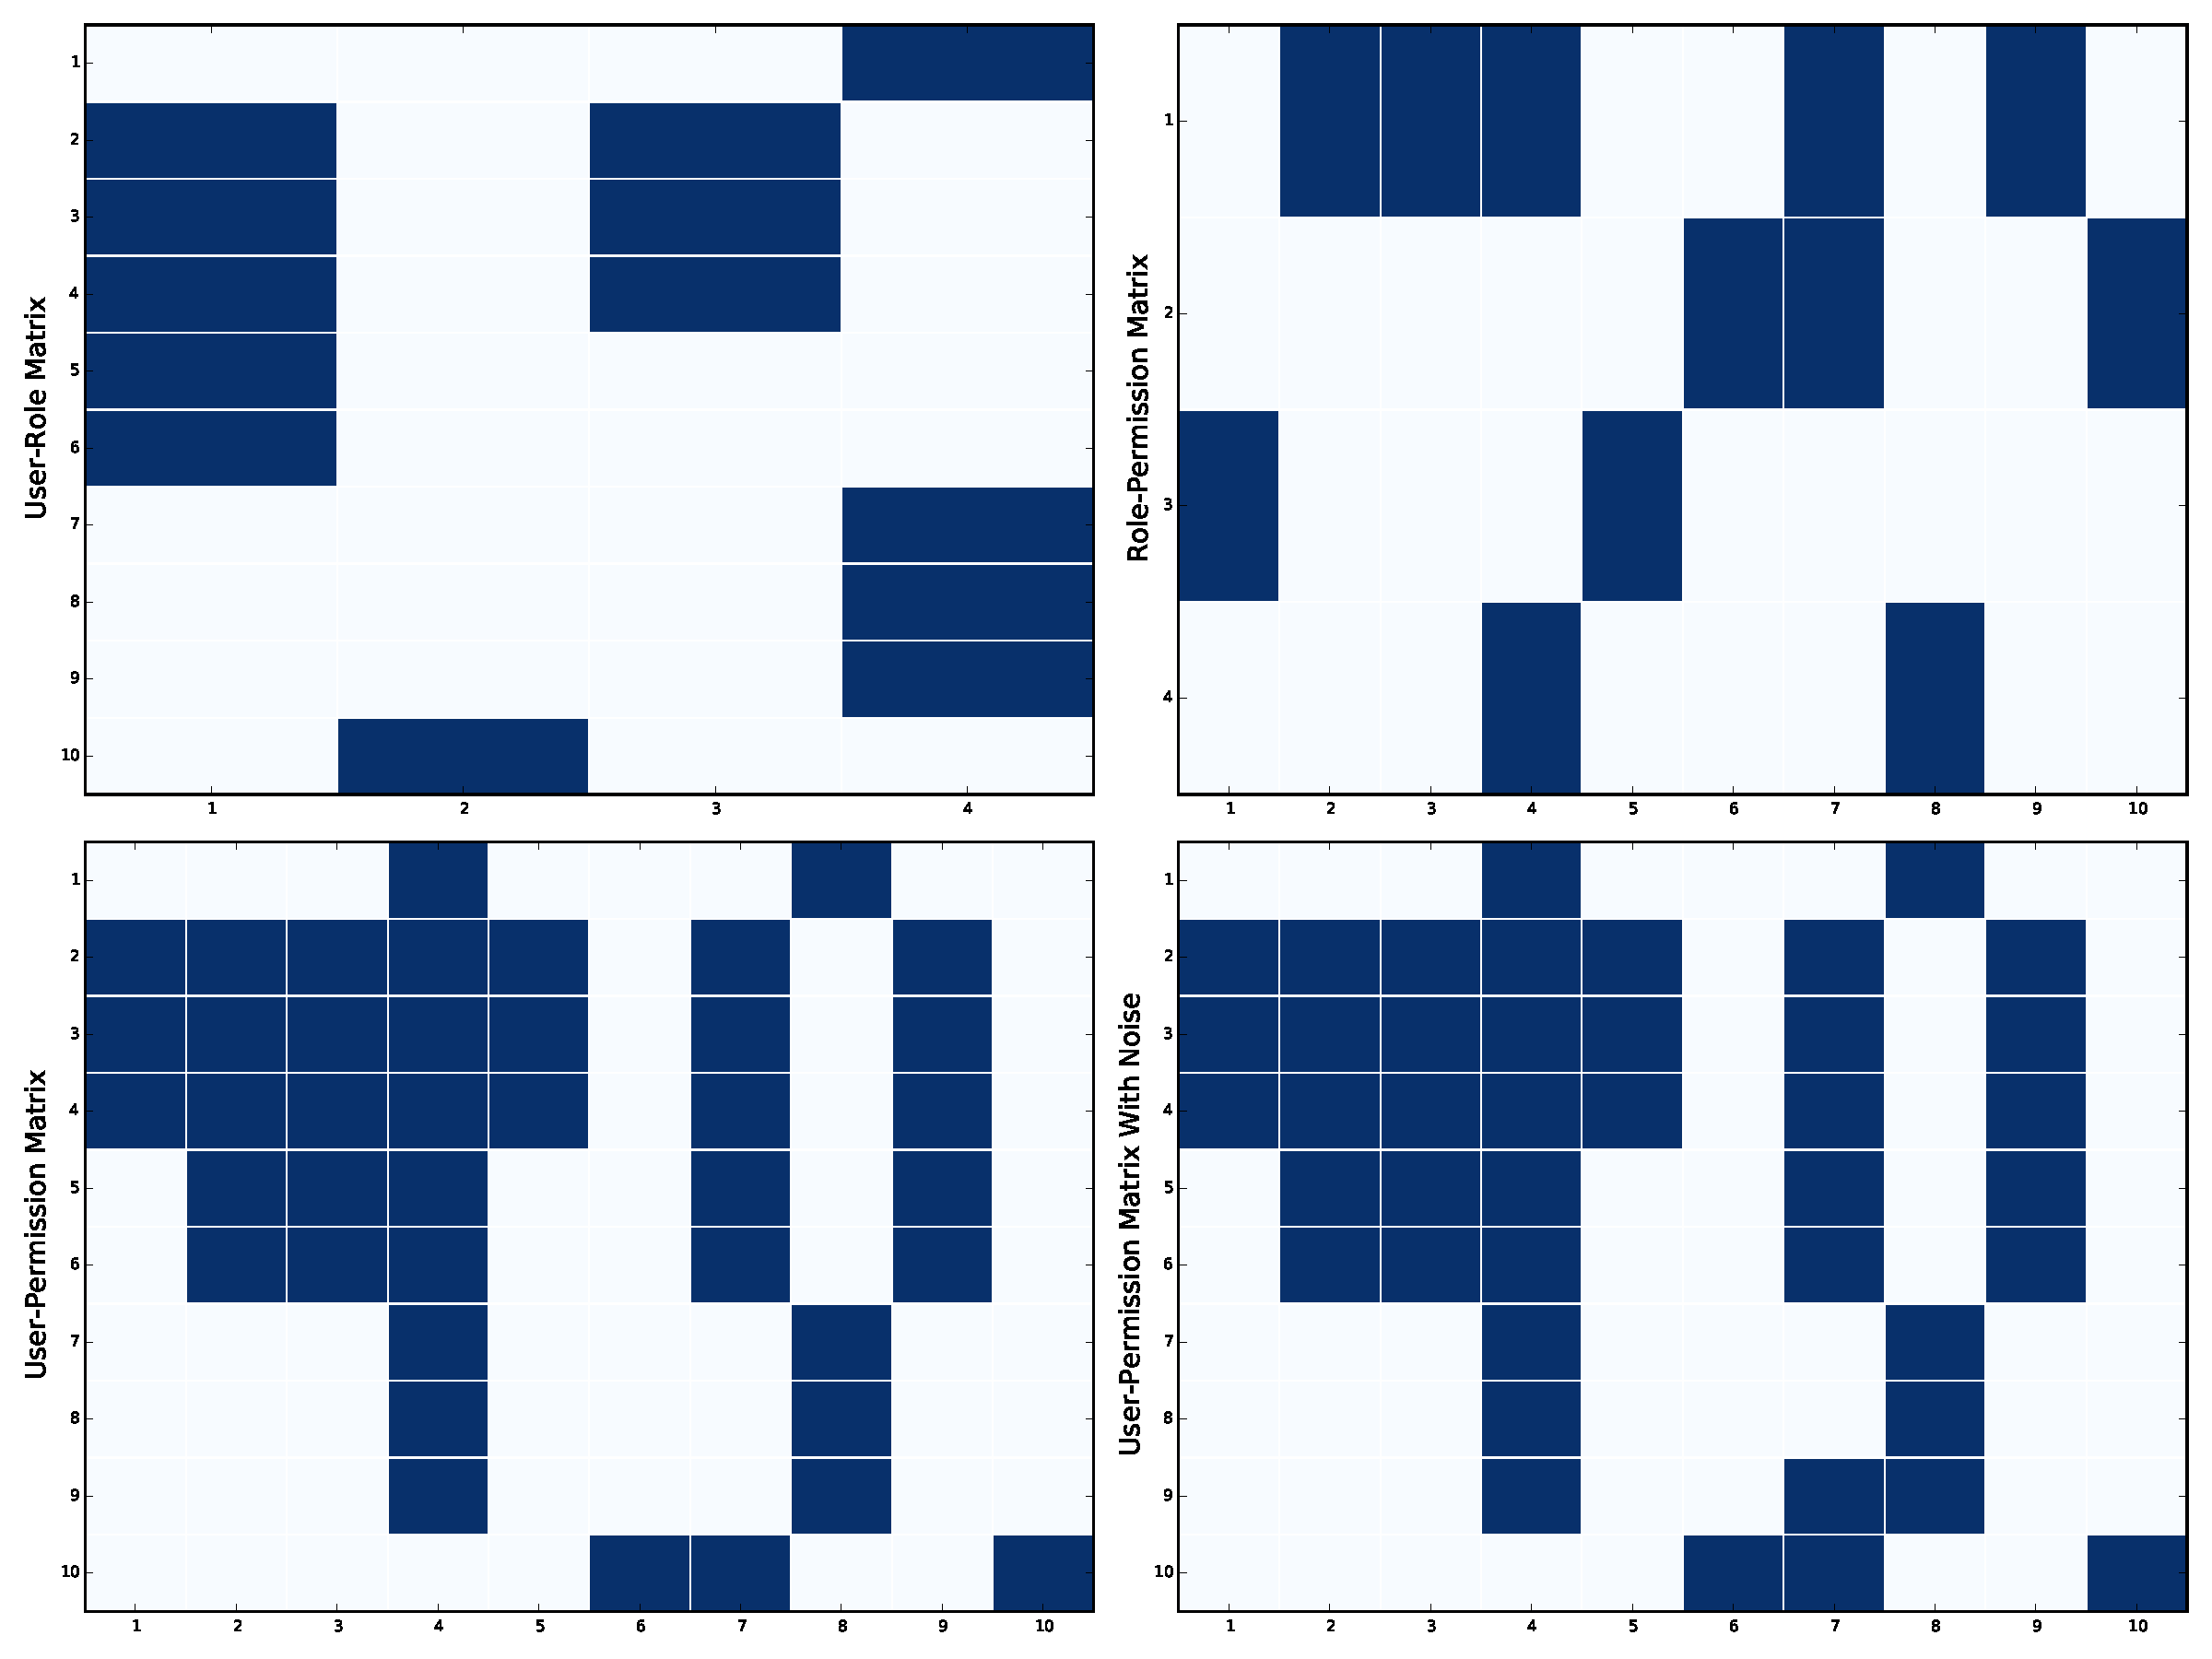
\includegraphics[scale=0.3]{./Figures/dataset1}
        \caption{DATASET 1: Role model of synthetic dataset 1 including User-Permission Matrix. From u.l. to l.r.: User-Role Matrix (Rows: Users, Columns: Roles), Role-Permission Matrix (Rows: Roles, Columns: Permissions), Resulting User-Permission Matrix (Rows: Users, Columns: Permissions), User-Permission Matrix with Noise (Rows: Users, Columns: Permissions)}
        \label{fig:dataset1}
    \end{figure}
    \clearpage
}

\afterpage{
    \begin{figure}[!htb]
        \centering
        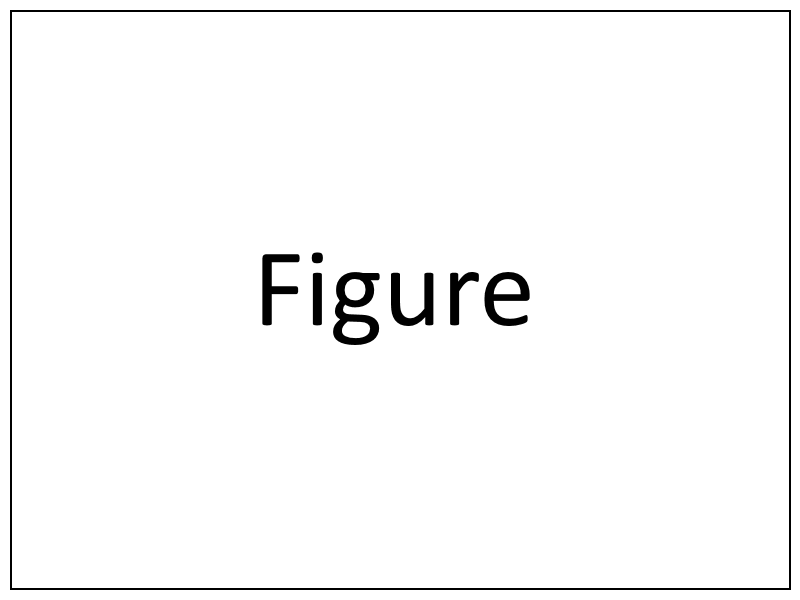
\includegraphics[scale=0.3]{./Figures/dummy}
        \caption{HEALTHCARE DATASET: User-Permission Matrix (Rows: Users, Columns: Permissions)}
        \label{fig:healthcare}
    \end{figure}
    \clearpage
}

\newpage
\section{Experiments with Evo-RoleMiner}
\hl{SECTION UNDER CONSTRUCTION}\\
The experiments have been divided into several phases, where the results of one phase lead to the setup of the experiments in the next phase.\\
In the first phase single objectives introduced in section \ref{sec:optimizationCompleteness}, \ref{sec:optimizationComplexity} and \ref{sec:optimizationComprehension} are set as fitness function in the Evo-RoleMiner. This phase was executed to validate the implementation of the objective functions, which are combined at a later stage, and to analyse the impact of these objectives to each other. The findings lead to the setup in phase two, where the actual fitness functions for the Basic-RMP, Min-Edge-RMP and Interference-RMP (see section \ref{sec:fitnessFunctions}) are used in the Evo-RoleMiner.\\
All experiments have been executed ten times and started with a random start-population. The experiments have been executed on the healthcare dataset (see Figure \ref{fig:healthcare}) and on a synthetic dataset generated by the data generator (see Figure \ref{fig:dataset1}).

\import{chapters/}{10_Phase1.tex}
\import{chapters/}{10_Phase2.tex}
\import{chapters/}{10_Phase3.tex}
\import{chapters/}{10_Phase4.tex}
\import{chapters/}{10_Phase5.tex}
\import{chapters/}{10_Phase6.tex}

\section{Experiments with Evo-RoleMiner$M$}
\hl{SECTION UNDER CONSTRUCTION}\\
\subsection{Setup}
\subsection{Measures}

\section{Experiments with Co-Evolution}
\hl{SECTION UNDER CONSTRUCTION}\\
\subsection{Setup}
\subsection{Measures}

\iffalse
\section{Experiments with Human Interaction}
\subsection{Setup}
\begin{itemize}
    \item Number of turns
    \item Random Start-population
    \item Fixed Start-population
\end{itemize}
\subsection{Measures}
\begin{itemize}
    \item Fitness (Min, Max, Avg)
    \item Time complexity
    \item Space complexity
\end{itemize}
\fi
